\documentclass{CLGPY}

\newtheorem{thm}{定理}

\newif\iffastcompile
\ifdefined\FASTCOMPILE
    \fastcompiletrue
\else
    \fastcompilefalse
\fi

\input{set/lstset.tex}%代码设置，定义了用来排版LaTeX代码的latexcode环境
%\input{set/fontset.tex}%字体设置
\input{set/shuoming.tex}%为了写说明文档而定义的几个命令

%--------------------------使用说明----------------------%
%注：\juanqi、\title、\author三条命令必须要有，不然系统会终止编译
\juanqi{X}{X}%卷期填写，命令\juanqi{<卷>}{<期>}
\title[]{网球拍效应的非线性动力学分析、实验与模拟}%标题填写，命令\title[<想要出现在奇数页页眉的标题，若缺省则默认为正式标题>]{<正式标题>}
\author[夏筠霖，等]{夏筠霖\textsuperscript{1}, 董\kern\ccwd 灏\textsuperscript{2}, 蒋程源\textsuperscript{3}}%作者填写，命令\author[<想要出现在奇数页页眉的作者，若缺省则默认为正式作者>]{<正式作者>}
\institute{{云南大学{\kern.5\ccwd} 物理与天文学院，云南{\kern.5\ccwd}昆明 650504}}%机构填写，命令\institute{<机构>}

\begin{document}
    \maketitle%生成题名页并修改题名页页眉

    \sxrq{2026--7--3}{2026--6--26}%收稿、修改日期，命令\sxrq{<收稿日期>}{<修改日期>}
    \jjxm{基金（xxxxxxxx）资助}%基金项目，命令\jjxm{<基金项目>}
    \zzjj{夏筠霖（2006 —），男，广东广州人，云南大学物理系本科生，主要从事物理方面的工作.\ts{（第一作者）}}%第一作者简介，命令\zzjj{<第一作者简介>}
    \txzz{X X，E–mail: \url{XXXXX@ynu.edu.cn}}%通讯作者，命令\txzz{<通讯作者>}

    \begin{abstract}%中文摘要环境
        本篇文章主要聚焦网球拍定理的理论、实验和仿真，理论方面主要依靠非线性动力学相分析，实验室主要利用刚体以及上面的角速度传感器，进行固联坐标系方面的角速度测量，并与理论预测进行对比，模拟方面考虑多种不同的初值问题积分方法，并结合此问题的特殊性指出每个方法的局限性以及适用场景，为未来可能存在的各种应用提供理论叙述和仿真分析案例.
    \end{abstract}
    \keywords{非线性动力学、相分析、初值问题、高阶算法、自适应步长、辛积分、刚体动力学}%中文关键词命令

    \xinxi{O 4–1\ts{(参照:\url{http://www.ztflh.com}})}{\bzx{A}{作者抄写}}{\bzx{1000-0712}{作者抄写} \bzx{XXXXXX}{编辑填写}}{\bzx{10.16854/j.cnki.1000-0712.}{作者抄写} \bzx{XXXXXX}{编辑填写}}%一些必要信息填写,命令\xinxi{<中图分类号>}{<文献标识码>}{<文章编号>}{<【DOI】>}

    \begin{multicols}{2}%以下部分内容采用双栏排版
        刚体自由转动的研究是经典力学中的重要研究内容之一，其运动规律被广泛应用于航空航天和机械工程相关领域，此问题具有相当完备的理论框架，即可以显式写出决定系统演化的运动方程，但是我们仍然对于自由转动的刚体的运动形式抱有很大误解，并且在现有数学框架下无法精确求解高维耦合自治方程的问题常常被许多人忽略，这些问题共同导致了网球拍效应给大多数第一次接触相关问题的人带来了困惑，这也是书写本文章的主要动机之一.
        
        关于刚体的转动稳定性的理论研究我们主要从20世纪中后期开始介绍，随着实验技术的发展，不少研究人员通过投掷网球拍、较重的卡片、书本以至于手机等具有三个不同主惯性矩的物体观察到意料之外的现象，主要体现于当他们开始绕中间主惯量轴（中间轴，即主转动惯量第二大的轴）抛出物体时，其姿态会周期性发生$180^\circ$的翻转，而不是像人们预期一样的绕主惯量轴的转动在无外力矩下理论上发生的恒定转动，此外，绕另外两个主惯量轴的转动却能够维持恒定转动，说明这个现象的奇异性就锁定在了绕中间轴的转动上，尤其是欧拉运动方程呈现的符号上的对称性更让人对中间轴这个看似普通的主惯量轴下隐藏的物理本质感到新奇.
        
        1985年，苏联宇航员弗拉基米尔·贾尼别科夫（Vladimir Dzhanibekov）在空间站进行实验时，注意到一枚旋转螺母在失重环境下会周期性翻转，该实验视频后来广泛传播，使这一现象再次受到关注，因此网球拍效应也常被称为“Dzhanibekov效应”或“贾尼别科夫效应”。该现象并非新的物理规律，而是中间轴定理在微重力环境下更加直观的实验体现，实际上，他们观察到的失重环境下观察这样的转动本质上与在地球上抛出物体后跟随质心坐标系观察等效，因为重力的作用是可以近似等效在质心上\footnote{网球拍远小于地球，质心和重心重合，此外，实际上在太空中的人也受到了重力，只不过由于以上的原因他们会感知不到重力的效果}.
        
        我们先给出网球拍效应（Tennis Racket Effect）的描述，网球拍效应本质是一个自由转动的刚体展现出的动力学现象，网球拍（及其类似物）在空中手柄本身转动了一周（$2\pi$）之后，网球拍会绕平行于手柄的轴转半圈因为网球拍是这个现象的主要展示载体以及在网络媒体上常常出现网球拍投掷产生了这样的现象，常称此现象为网球拍定理.
        
        这个现象在论文\cite{1991_Ashbaugh,2015_Cushman_BOOK}中做出了数学讨论，并取得了卓越的成果，但是也做出了不可忽视的妥协，那就是他们研究的对象是$I_1+I_2 \simeq I_3 $的特殊情况，这样的限制使他们的研究结果能够描述的范围十分有限.
        
        本问题的主要重心在于如何处理欧拉方程这个互相耦合的高阶自治非线性方程，自牛顿时代开始，高阶非线性方程就是常见的难以处理的难题，其中最具代表性的就是三体问题，这个问题横跨整个数学物理发展史，以欧拉为代表的一众世界著名数学家都无法处理.突破出现在19世纪末，法国数学家昂利·庞加莱（Henri Poincaré）在研究三体问题时发现这类系统难以以解析的方式进行求解，并且他们的行为对初始条件极为敏感，即长期运动难以预测，故他因启用图像的方式对系统整体的走势进行研究，并且着重聚焦于那些特征点和轨迹（固定点、零斜率线等），他在此后做出的一系列贡献使他被广泛认为是现代拓扑学、非线性动力学和混沌理论的主要奠基人.本文将延续这种思路，从非线性动力学基础理论\cite{2024_Strogatz_BOOK}出发，采用图像的视角分析出现在网球拍效应中的非线性现象.
        
        实际上本问题在\cite{1991_Ashbaugh}的论文中已经提供了使用雅克比椭圆函数描述的解析解\footnote{Abramowitz and Stegun, 1964; Gradshteyn and Ryzhik,1980; Tricomi, 1953; Rauch and Lebowitz, 1973，Ashbaugh的文章太早了，其引用信息使我找不到椭圆函数的出处，此处就直接把原文的引用搬来了}，但是即使如此仍有文章研究这个问题，主要是因为椭圆函数过于复杂，多个中间量互相嵌套，物理图像不清晰，只有最开始的Ashbaugh这篇文章较为仔细的描述了椭圆函数，之后大多数文章就只是提一下椭圆函数，而不继续往下说明了。
        
        本文主要聚焦这篇2017年的论文\cite{2017_VanDamme}中部分的结论，给出网球拍定理的较为完整的分析路径，包括对于中间轴定理的理论分析、实验与数值模拟和对于网球拍效应的非线性动力学分析，随后我们将给出一个\cite{2017_VanDamme}中的理论来描述网球拍效应的效果，对理论上的解的表达式做了数值模拟，最后我们将直接对决定这个系统演化的方程即欧拉动力学方程的完整形式进行数值模拟，并采用多种数值方法验证这个理论是否正确。
        
        论文\cite{2017_VanDamme}部分地使用了非线性动力学的方法，为人们理解网球拍效应做出了重大贡献，但是仍然存在些许不足，主要体现在他虽然引入了朗道在书本\cite{Landau_2013_BOOK}中得到的引入了欧拉角的欧拉动力学方程的化简后的形态，将系统从六阶降到了三阶，并且进一步降到了二阶，但是VanDamme将两个变量分开讨论，以欧拉角和欧拉角的变化率作为坐标轴强行绘制相图，这样得到的结果就是$\psi$角的变化在$\cos\theta = 0$处难以描述，$\theta$和$\dot{\theta}$更是不构成自治系统，绘制的相图无法直接用非线性动力学分析，并且其论文中虽然提到了鞍点和中心点，但是对于这两个固定点的分析欠佳，我们将在此论文中在一定程度上弥补这些缺憾.
        
        ,,,,引言部分不需写标题，即不写“引言”二字．参考文献序号按其在文中出现的顺序编排，文中引用处用上标\cite{xingshinianfenlun,li2000yi}，3个以上用连字符\cite{xingshinianfenlun,li2000yi,CTEX}．全文数字、西文用Times New Roman(\ts{已设定})，句号用实心点


		\section{数学物理模型建立}
		\subsection{欧拉角约定}
		我们先作一个核心约定，那就是欧拉角的约定，为了方便与参考文献对比，以及公式形式和理论使用的统一性，我们将随从文章\cite{2017_VanDamme,Landau_2013_BOOK}的约定，按照\autoref{fig:ueler-angle} \autoref{fig:axes}的形式使用欧拉角：
		\begin{center}
8.			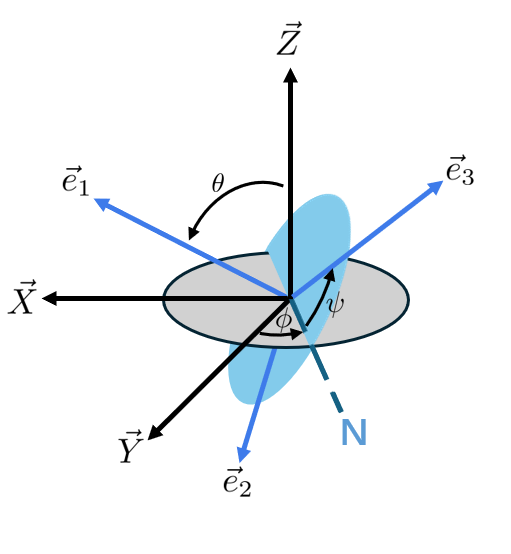
\includegraphics[width=8cm]{./fig/euler-angle.png}
			\captionof{figure}{欧拉角（Euler angles），黑色和蓝色圆盘仅为视觉辅助作用，请勿混淆. \label{fig:ueler-angle}}
		\end{center}
		\begin{center}
			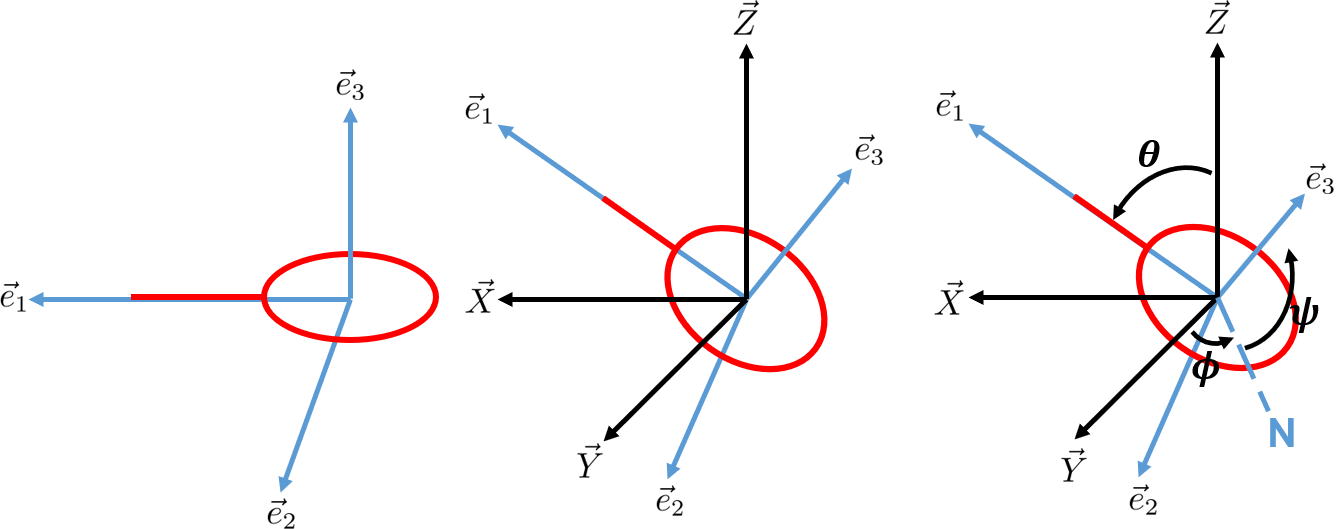
\includegraphics[width = 8cm]{./fig/axes.png}
			\captionof{figure}{带上网球拍后的坐标的建立，其中蓝色为固联坐标系，黑色为质心系，红色为网球拍. \label{fig:axes}}
		\end{center}
		同时我们认为这也是最为直观的欧拉角约定，简要来说，$\theta$角和$\phi$共同来决定拍柄的朝向，随后$\psi$角单独决定其翻面的情况，并且$\vec{e}_1,\vec{e}_2,\vec{e}_3$（三个固联坐标系上面的基矢量）对应于$I_1<I_2<I_3$（三个主转动惯量）
		
		\subsection{符号约定与模型假设}
		\begin{center}%使表格居中，不使用浮动体环境
			\captionof{table}{符号约定}%表名置于表格上方
			\begin{tabular}{>{\small}l>{\footnotesize}l}%列格式说明：两列，左对齐，同时使用array宏包提供的>{<内容>}（表示把<内容>插入其后所在列的开头）设置各列字体尺寸
				\toprule %画表格顶部粗线
				\textbf{符号} & \textbf{\small 定义} \\%第一列标题加粗，第二列标题在加粗的同时把字体尺寸设为small，然后用\\换行
				\midrule %画表格中间分隔线
				$\theta, \phi ,\psi$   	&   欧拉角\:(rad)   \\
				$M$   					&   总角动量\:(Kg$\cdot$mm$^2 \cdot$s$^{-1}$)   \\
				$E$   					&   质心坐标系中的总转动动能\: ( $\mu$J )   \\
				$ M_1,M_2,M_3 $  	 	&   主轴方向上的角动量\: (Kg$\cdot$mm$^2 \cdot$s$^{-1}$)   \\
				$I_1<I_2<I_3$   		&   主转动惯量\: (Kg$\cdot$mm$^2$)   \\
				$\varepsilon,\vec{\varepsilon}$   &   小量\: (rad$\cdot$s$^{-1}$)   \\
				$\omega,\vec{\omega}$   &	角速度\: (rad$\cdot$s$^{-1}$)   \\
				\bottomrule %画表格底部粗线
			\end{tabular}
		\end{center}
		
		以下为本篇大多数时候都默认使用的假设，之后可能会考虑其他情况，在那些特殊的部分，我们会提前声明.
		
		\begin{description}
			\item[假设1]
			认为物体是刚体.
			\item[假设2]
			不考虑空气阻力.
			\item[假设3]
			重心与质心重合.
		\end{description}
		
		\section{不稳定性分析}
		我们此处主要聚焦于一个关键的旋转情况下的稳定性分析，即当网球拍在绕中间轴旋转的时候不稳定性，此被称为中间轴定理.
		
		\begin{thm}[中间轴定理]
			
			{\kaishu 当刚体绕转动惯量最大或最小的主轴（第一、第三主轴）旋转时保持稳定，而绕中间轴（第二主轴）旋转时会产生不稳定性。}
			
		\end{thm}
		
		这个定理是网球拍定理的基础，它指出网球拍非同寻常的旋转的来源，为了说明这个定理，我们先做一些基础分析，使用最基础的欧拉动力学方程，即用固联坐标系下的各个轴的角速度$\omega_1,\omega_2,\omega_3$表示的欧拉方程\:($\dot{\omega}$代表角速度分量对时间求一阶导)
		\begin{align}
			&I_1\dot{\omega}_1-(I_2-I_3)\omega_2\omega_3 = \tau_1 \notag \\
			&I_2\dot{\omega}_2-(I_3-I_1)\omega_3\omega_1 = \tau_2 \\
			&I_3\dot{\omega}_3-(I_1-I_2)\omega_1\omega_2 = \tau_3 \notag
			\intertext{其中整个刚体相对于质心所受的合外力矩\: $\tau_i = 0 \:(i = 1,2,3)$}
			&I_1\dot{\omega}_1=(I_2-I_3)\omega_2\omega_3 \notag \\
			&I_2\dot{\omega}_2=(I_3-I_1)\omega_3\omega_1 \label{equ_ueler} \\
			&I_3\dot{\omega}_3=(I_1-I_2)\omega_1\omega_2 \notag
		\end{align}
		这就是我们整个讨论中最基础的运动方程，其中显而易见的是，当角速度只沿着一个轴的时候，在\autoref{equ_ueler}中三个方程的等号右边全部为零，所以三个角速度分量全都不发生变化，旋转过程中不改变整体的状态，但是如果存在扰动的话，三个轴就需要分别讨论了。
		
		我们先看绕最小轴的旋转受到了微小扰动是否会保持稳定（在稳定状态周围产生振荡），首先假设若绕最小轴的旋转为：
		\begin{gather*}
			\omega_0 = \frac{M_1}{I_1} \\
			\intertext{受到微小扰动{\boldmath$\epsilon_0$}(小量|{\boldmath$\epsilon_0$}|$\ll M_1$，|{\boldmath $\dot{\epsilon}_0$}|也为小量)} 
			\omega_1 = \omega_0+\epsilon_1 \\
			\omega_2 = \epsilon_2 \\
			\omega_3 = \epsilon_3 \\
			\intertext{先仅考虑开始很小一段时间内的情况，代入方程\eqref{equ_ueler}的三个方程，其第一个量为：}
			I_1\dot{\omega}_1 = (I_2-I_3)\epsilon_2\epsilon_3 \approx 0 \\
			\intertext{二阶小量我们近似为零,故认为当扰动开始很小的时候$\omega_1 = C(constant)$,现在看其他的量}
			\dot{\epsilon}_2 \approx C\frac{I_3-I_1}{I_2}\epsilon_3 \\
			\dot{\epsilon}_3 \approx C\frac{I_1-I_2}{I_3}\epsilon_2 \\
			\intertext{看这两个式子，我们先做下面的简记约定：}
			-C^2\frac{(I_3-I_1)(I_1-I_2)}{I_2I_3} = k > 0
		\end{gather*}
		\begin{gather}
			\intertext{那两个式子中，上式左右求导后代入下式的$\dot{\epsilon}_3$，下式左右求导后带入上式的$\dot{\varepsilon}_2$}
			\ddot{\varepsilon}_2 +k\varepsilon_2 \approx0 \notag \\
			\ddot{\varepsilon}_3 +k\varepsilon_3 \approx0 \label{equ_stable} 
		\end{gather}
		这里可以看到，$\varepsilon_2,\varepsilon_3$会近似以$\sqrt{k}$为周期做简谐运动，并且初值条件$\varepsilon_{i0},\dot{\varepsilon}_{i0}\:(i = 1,2,3)$都是小量，说明$\varepsilon_2,\varepsilon_3$可以被认为全程都是小量，所以$\omega_1$可以被认为全程近似不变而非暂时不变\footnote{此处可以用递归的论述完整逻辑链路，不过这些过于繁琐，我们此处就不展示了}，这一系列过程导致整个系统是稳定的，这个结论可以通过对初始的欧拉方程进行数值模拟来得到，模拟与实验的结果对比参看\autoref{fig:minimal-axis}
		
		\begin{center}
			\includegraphics[width = 8cm]{./fig/minimal_axis.png}
			\captionof{figure}{数值模拟以及实验数据对比-最小轴，关于实验的设置、实验数据的处理、算法选择、结果分析、误差分析和能量分析，我们将放在后文实验说明部分进行详细阐述. \label{fig:minimal-axis}}
		\end{center}
		
		我们可以套用这个分析过程到其他情况，过程此处我们不多赘述，详细的分析过程参见参考文献1，但是有趣的事情是，我们最终得到的结果出现了分歧，如果一开始是绕$I_3$所在的轴旋转，那么整个系统是稳定的，结果与开始绕$I_1$的轴旋转无异，但是如果一开始是绕$I_2$所在的轴进行旋转，我们得到如下结果：
		\begin{gather*}
			\intertext{在开始很小的一段时间内，$\omega_2 \approx C_2$}
			\ddot{\varepsilon}_1 +k\varepsilon_1 \approx 0  \\
			\ddot{\varepsilon}_3 +k\varepsilon_3 \approx 0 \\
			\intertext{其中：}
			k = -C^2\frac{(I_3-I_2)(I_2-I_1)}{I_1I_3}<0 \\
			\intertext{这说明在开始很小一段时间内，$\epsilon_1,\epsilon_3$会呈指数增长，鉴于两个方程的形式一样，我们挑选其中一个分析，另外一个同理.}
			\intertext{以下是这个方程的解:}
			\varepsilon_1 = C_1e^{\sqrt{-k}t}+C_2e^{-\sqrt{-k}t} \\
			\intertext{其中：}
			C_1 = \frac{\varepsilon_{10}+\frac{\dot{\varepsilon}_{10}}{\sqrt{-k}}}{2} \\
			C_2 = \frac{\varepsilon_{10}-\frac{\dot{\varepsilon}_{10}}{\sqrt{-k}}}{2}
		\end{gather*}
		
		可以看出，在开始的一小段时间内，$\varepsilon_1,\varepsilon_2$会以指数形式增长，随后$\omega_2$会出现变化，导致整个运动脱离了开始的状态，这种情况就像是放在平滑山丘顶端的小球，虽说理论上是可以在此保持平衡，但是受到任何形式的干扰都会使其脱离原来的平衡点，这就是整个系统的不稳定平衡点，于是，中间轴定理就基本地证明完了，以下是对其进行的数值模拟和实验数据对比（\autoref{fig:intermediate-axis}）
		
		\begin{center}
			\includegraphics[width = 8cm]{./fig/intermediate_axis.png}
			\captionof{figure}{数值模拟以及实验数据对比-中间轴. \label{fig:intermediate-axis}}
		\end{center}
		
		\section{非线性动力学分析}
		\subsection{前置分析}
		以下是一个最被认为最开始描述这个现象的论文的作者对其的描述，就是其运动轨迹可以看作两个3维相空间两个球(椭球)的交线\cite{1991_Ashbaugh}，这个描述被后来的一些文献提到并作为开头对现象的解释，我们也将以此作为开头，并将在后文中使用这个图像结合中间轴定理处理一个棘手的问题：雅可比矩阵为全零矩阵的鞍点如何在一定程度上定性确认其不会分叉.
		\begin{align}
			& E = \frac{1}{2}(\frac{M_1^2}{I_1}+\frac{M_2^2}{I_2}+\frac{M_3^2}{I_3}) \label{equ:E} \\
			& M^2 = M_1^2+M_2^2+M_3^2 \label{equ:AM}
		\end{align}
		\begin{center}
			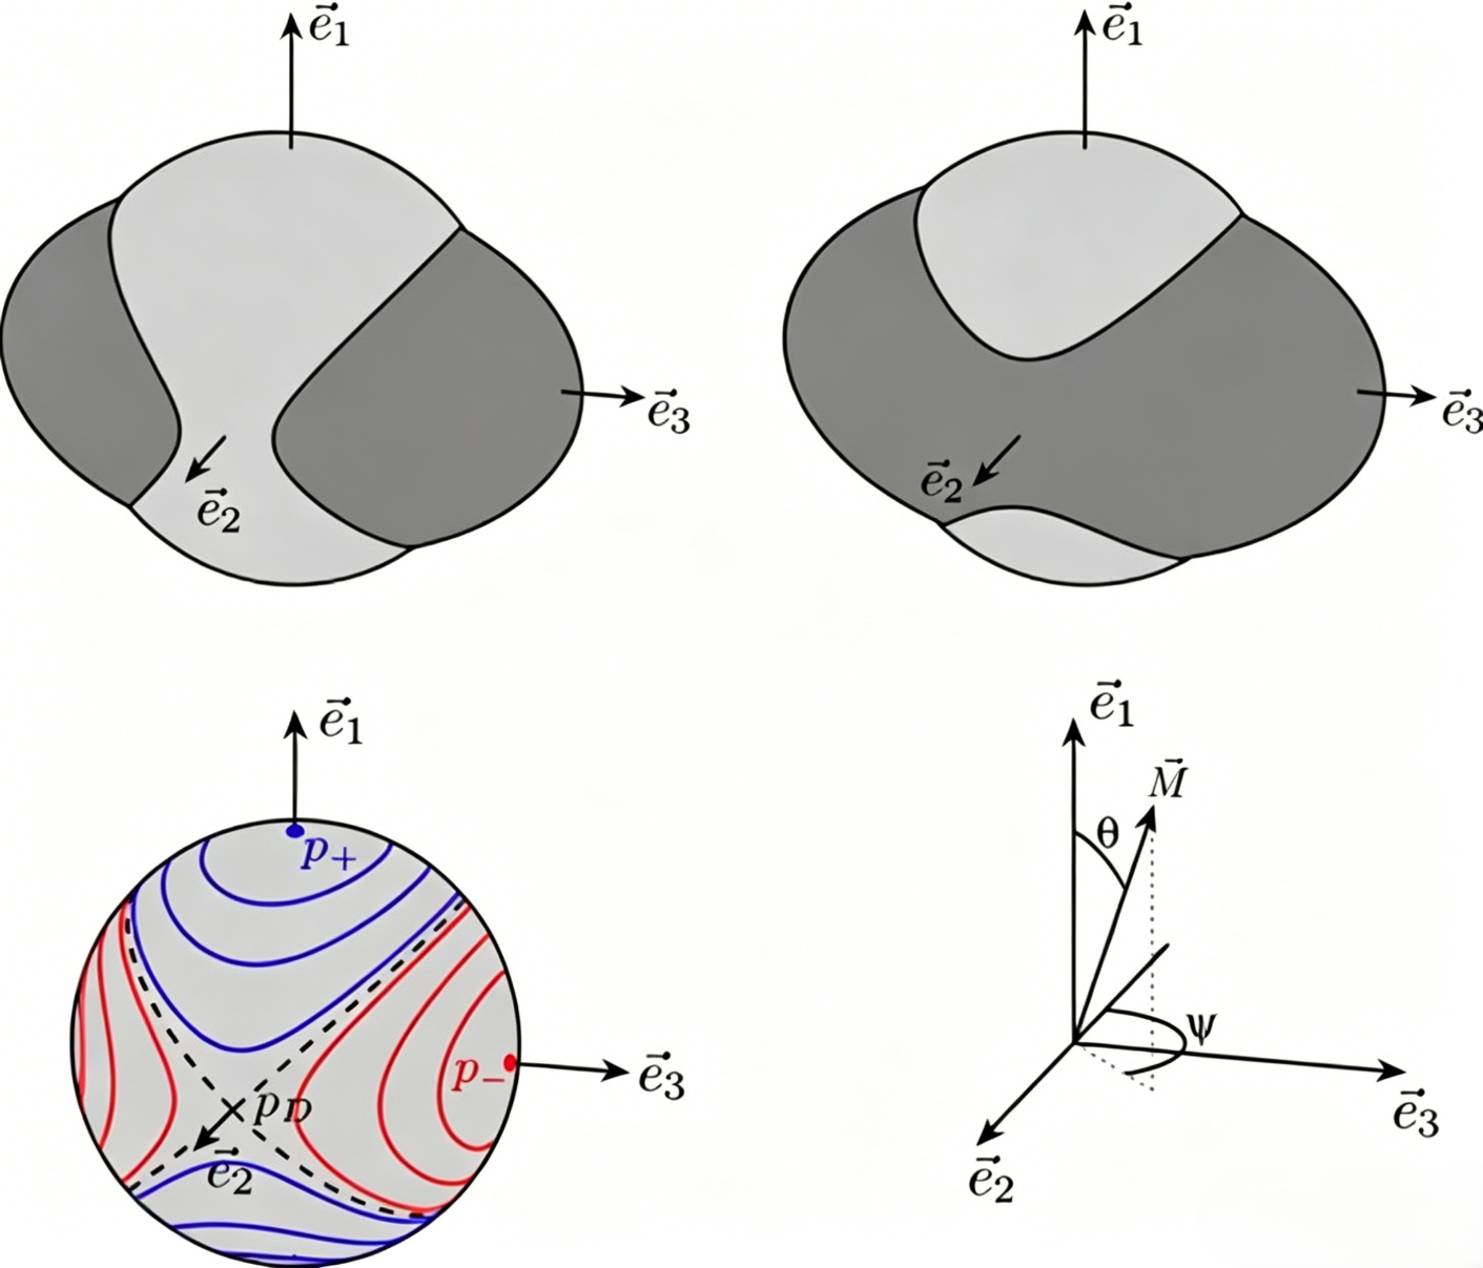
\includegraphics[width = 8cm]{./fig/E_AM_intersection.png}
			\captionof{figure}{能量守恒和角动量守恒以及其相交的轨道，图像来自\cite{2017_VanDamme}，这个图像主要描述的是：以三个主轴方向上的角动量为坐标轴，能量守恒和角动量守恒两个限制条件形成一个椭球面和一个球面，两球面相交可以得到总角动量在固联坐标系中的演化形式，红色为谐振状态，对应左上的图，蓝色为旋转状态，对应右上的图.右下的图片说明了此图的演化和欧拉角的对应关系，此外严格上讲这里的$\psi$角与原来的欧拉角差了一个$\frac{\pi}{2}$，不影响分析. \label{fig:E_AM_intersection}}
		\end{center}
		此外，我们也可得到两种形式的临界点，此处我们用一个参数$\gamma = \frac{2I_2E}{M^2} - 1$来描述它，从球面之前相切的情况可以看出：$\gamma < 0$ 谐振状态，红色轨迹，对应左上的图，$\gamma > 0$ 旋转状态，蓝色轨迹，对应右上的图片，我们此处只是复述了\cite{2017_VanDamme}的结果.
		
		\subsection{相图的绘制与分析}
		在\autoref{fig:E_AM_intersection}中的左下角的图片与一个2维相平面投影到了一个球体当中的形式十分相似，从非线性动力学(主要参考书\cite{2024_Strogatz_BOOK})的角度看，就好像4个中心点(centers)围绕一个鞍点(saddle points)，之后我们会说明这一点，此处我们先处理欧拉动力学方程\autoref{equ_ueler}，带入欧拉角和总的角动量把其变成完整形式\cite{1991_Ashbaugh}\cite{2017_VanDamme}\cite{Landau_2013_BOOK}。
		
		\begin{align*}
			& \dot{\theta} = M(\frac{1}{I_3}-\frac{1}{I_2})\sin\theta\sin\psi\cos\psi \\
			& \dot{\phi} = M(\frac{\sin^2\psi}{I_3}+\frac{\cos^2\psi}{I_2}) \\
			& \dot{\psi} = M(\frac{1}{I_1}-\frac{\sin^2\psi}{I_3}-\frac{\cos^2\psi}{I_2})\cos\theta 
		\end{align*}
		
		这个形式是接下来讨论的基础形式，可以看出$\phi$这个变量是恒单调递增的，这个性质有利于我们后续理解运动，到此其实已经可以开始处理了，但是为了避免繁琐的设置转动惯量的大小和相对关系，并且突出其物理实质，我们引入以下参量：
		
		\begin{align*}
			a = \frac{I_2}{I_1}-1 \qquad
			b = 1 - \frac{I_2}{I_3} \qquad
			\gamma = \frac{2I_2E}{M^2} - 1 \\
			0< a < +\infty \qquad
			0< b < 1 \qquad
			-b\leq \gamma \leq a
		\end{align*}
		
		$\gamma$为连接\autoref{fig:E_AM_intersection}与后续分析的桥梁，$a,b$主要描述的是系统的对称性(转动惯量间的相对大小)，因为我们认为决定系统变化的是转动惯量的相对大小而不是绝对大小.
		
		为了绘制相图并且避免复杂的分析，我们希望将将系统降至二维，这样就可以绘制其相图并且利用非线性动力学里面的一些理论工具，此处注意到：$\phi$角是严格单调递增的，可以在此处用$d\phi$消去$dt$，把$\phi$角的变化作为时间变量的替换，可以认为其就是时间尺度做了一些不规则拉伸，随后带入这几个参量，省去一些操作步骤，我们得到：
		
		\begin{align}
			& \frac{d\theta}{d\phi} = -\frac{b\sin\theta\sin\psi\cos\psi}{1-b^2\sin^2\psi} \\
			& \frac{d\psi}{d\phi} = \frac{(a+b\sin^2\psi)cos\theta}{1-b\sin^2\psi} 
			\label{equ_dpsi} \\
			& \gamma = a-\sin^2\theta(a+b\sin^2\psi) 
		\end{align}
		
		我们对前两个方程组绘制相图，可以得到以下结果；
		
		\begin{figure*}[!t]
			\centering
			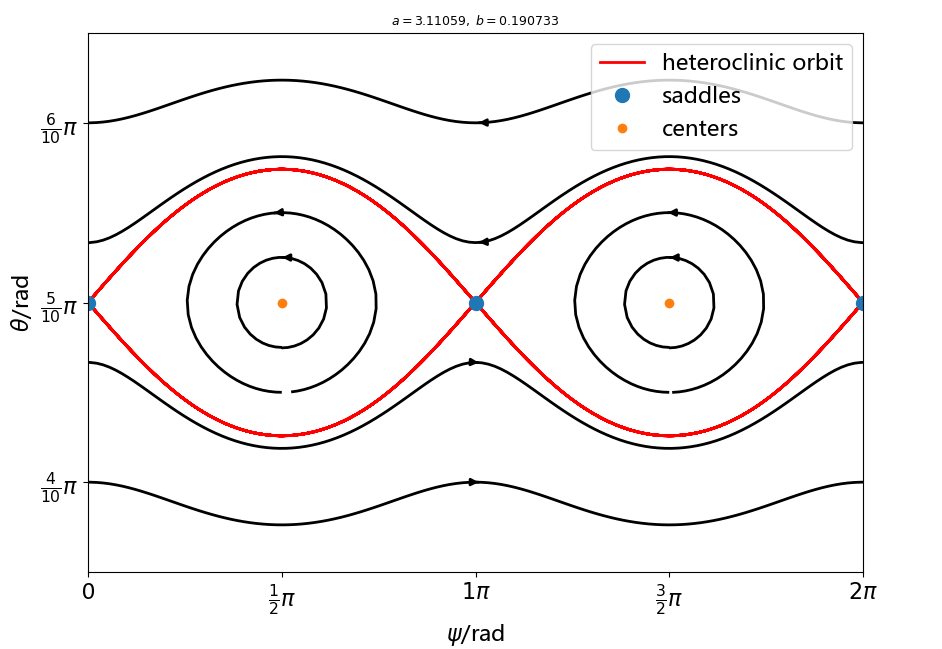
\includegraphics[
			width=\textwidth,
			keepaspectratio
			]{./fig/phase_portrait.png}
			\caption{关于$\psi$与$\theta$的相图，参数使用的是本论文实验部分的实验对象。}
			\label{fig:phase_portrait}
		\end{figure*}
		
		我们先对这个相图做一些基本的理论工作，以确保相图性质的普适性，检查固定点(fixed points)的信息，以及是否存在分叉现象.
		
		首先在这个取值范围内有$(0,\frac{\pi}{2}),(\frac{\pi}{2},\frac{\pi}{2}),(\pi,\frac{\pi}{2})$为固定点，其他的点可以按照三角函数的周期性来扩展，所以我们就可以用这张图来分析$\psi = \pi$开始的运动，因为它们实际上是等价的，我们先计算其雅可比矩阵(\textit{\textsl{Jacobian matrix}})：
		
		\begin{align*}
		A_{(0,\frac{\pi}{2})} = A_{(\pi,\frac{\pi}{2})} = \begin{pmatrix}
			0 & 0 \\
			0 & 0 
		\end{pmatrix} \\
		A_{(\frac{\pi}{2},\frac{\pi}{2})} = \begin{pmatrix}
			0 & \frac{b}{1-b^2} \\
			\frac{a+b}{b^2-1} & 0
		\end{pmatrix}
		\end{align*}
		
		虽然上述雅可比矩阵都非常棘手，因为它们不在非线性系统的可以被线性分析的范围之内，但是我们在此指出，对于我们上面提到的中心点，这是一个可逆系统\cite{2024_Strogatz_BOOK}，即整个系统在$\phi \longrightarrow -\phi, y \longrightarrow -y$的时候形式保持不变，于是我们可以处理$(\frac{\pi}{2},\frac{\pi}{2})$点，因为雅可比矩阵说明它是一个线性中心点，系统是连续可逆的，根据书本\cite{2024_Strogatz_BOOK}的定理6.6.1：
		
		\begin{thm}[可逆系统的非线性中心点]
			
			{\kaishu 假设$x^\star = 0$是以下连续可微系统的一个线性中心点}
			
			\begin{align*}
				& \dot{x} = f(x,y) \\
				& \dot{y} = g(x,y)
			\end{align*}
			
			{\kaishu 在此基础上如果系统可逆，那么足够靠近原点的轨迹是闭合曲线}
		\end{thm}
		
		我们认为$()$，套用这个定理需要对系统做平移等操作，我们此处略去这些过程.
		
		对于鞍点，全零矩阵的特殊性需要进一步深入的数学分析，我们欢迎任何补充，此处我们不好用线性的理论进行分析，但这正是我们前面的工作起到效果的地方，我们现在先对齐\autoref{fig:E_AM_intersection}和\autoref{fig:phase_portrait}：
		
		\begin{align*}
			\intertext{有前面引入的参数$\gamma$以分划两种状态可以看出，当：}
			\theta = \frac{\pi}{2} ,\psi = \pi  \\
			\intertext{有：}
			\gamma = 0
		\end{align*}
		因为$\gamma = 0$是由初始条件决定的，说明在系统演化过程的一点$\gamma = 0$此后全过程都满足$\gamma = 0$，这说明其对应了至少2条轨迹，因为在\autoref{fig:E_AM_intersection}中存在两条$\gamma = 0$的两条轨迹，而在\autoref{fig:phase_portrait}中正好有两个异宿轨道从$(\pi,\frac{\pi}{2})$伸出，如前面的分析这两条轨迹必然也有$\gamma = 0$的特征，随后根据2维相图轨迹是唯一且不相交的性质，我们此处定性的将这两条轨迹对应上，这样整个相图\autoref{fig:phase_portrait}就可以认为是把\autoref{fig:E_AM_intersection}左下角的轨迹图展开平铺到平面上面的样子，这样其附近的运动应对应着\autoref{fig:E_AM_intersection}在$\gamma = 0$附近系统演化的轨迹，结合原本就有的方向特征，我们可以证明在$(\pi,\frac{\pi}{2})$附近其轨道与鞍点的轨道是完全一致的，如下图所示，同时我们结合中间轴定理，当初始完全围绕着中间轴旋转的时候$\gamma = 0$，故$(\pi,\frac{\pi}{2})$对应着绕中间轴旋转的初始条件，所以在$(\pi,\frac{\pi}{2})$附近的点的运动是不稳定的，且永远不可能到达此点本身（若到达此点，则系统到达固定点，系统就被固定了，不会继续演化，与理论矛盾），于是我们得到结论：这个点的行为和鞍点一模一样，于是我们形式上称之为鞍点.
		
		以上的结论不取决于三个参数$\gamma$的取值情况，同时只要$a, b\neq 0 $，相图所有固定点都不会发生分叉(bifurcation)，所以我们此处做出判断：相图在满足$I_1 < I_2 < I_3 $
		的情况下，只要坐标系妥当选择（不选择欧拉角存在歧义的点上），系统总存在类似的相图，只不过是有所拉伸或者单位不同.
		
		现在我们着手提取相图提供给我们的信息，首先我们可以看出不论是谐振状态还是旋转状态（采取了\autoref{fig:E_AM_intersection}中的分类方式：\autoref{fig:phase_portrait}中异宿轨道内的为谐振状态，对应\autoref{fig:E_AM_intersection}中的红色轨迹；\autoref{fig:phase_portrait}中异宿轨道外的为旋转状态，对应\autoref{fig:E_AM_intersection}中的蓝色轨迹），$\theta$永远只在一定范围内震荡，且每个周期之后它会回到原来的大小，而网球拍定理是研究$\psi$角转过一个$\pi$之后的行为，还是从鞍点附近出发，所以网球拍定理是研究从鞍点附近出发近似一个周期之后的行为，其中$\theta$正好近似回到起始值，说明$\theta$对刚体整体的旋转（即网球拍的手柄的旋转）没有贡献.剩下一个可以为刚体整体的旋转提供贡献的变量就是$\phi$，此处奠定我们后文的方向，说明$\phi$角转过近似$2\pi$以后$\psi$角大约转过$\pi$，如果能定量给出误差当然是最好的.
		
		幸运的是，我们此处有可以借鉴的前人的成果，它完整地描述了我们此处缺少的$\phi$角分析，即如下定理\cite{2017_VanDamme}：
		
		\begin{thm}[关于网球拍定理的微分方程有以下特性]
			对以下方程：
			\begin{align*}
				 \int_{\psi_0}^{\psi_f} f(a,b,&\psi,\gamma) d \psi = 2\pi \\
				 \psi_0 = \varepsilon& ,\qquad  
				\psi_f = \pi - \epsilon \\
				\intertext{其中：}
				f(a,b,\psi, \gamma) =  S&\frac{1 -b\sin^2\psi}{\sqrt{a+b\sin^2\psi}\sqrt{\gamma+b\sin^2\psi}} \qquad S = sign(\cos \theta) \\
				\intertext{推得有：} 
				 \varepsilon = \varepsilon_0 - &\frac{\gamma}{4b\epsilon_0} +O(\gamma^2). \\
				\intertext{$\varepsilon_0$是以下方程的解：}
				 \frac{\sqrt{1+\frac{b}{a}\sin^2\varepsilon_0} - \cos \varepsilon_0}{\sqrt{1+\frac{b}{a}\sin^2\varepsilon_0} + \cos \varepsilon_0}  &= e^{-2\sqrt{ab}[\pi+\arcsin(\sqrt{\frac{b}{a+b}}\cos \varepsilon_0)]}\\
				\intertext{$\varepsilon_0$解得：} 
				 \varepsilon_0 = e^{-\sqrt{ab}\pi} (2\sqrt{\frac{a}{a+b}}&e^{ -\frac{b}{\sqrt{1+b/a}} } + o(e^{-\sqrt{ab}\pi})) 
			\end{align*}
			\label{thm:TRE}
		\end{thm}
		
		以下是我们绘制的$\epsilon_0$的数值解可视化3D图：
		\begin{center}
			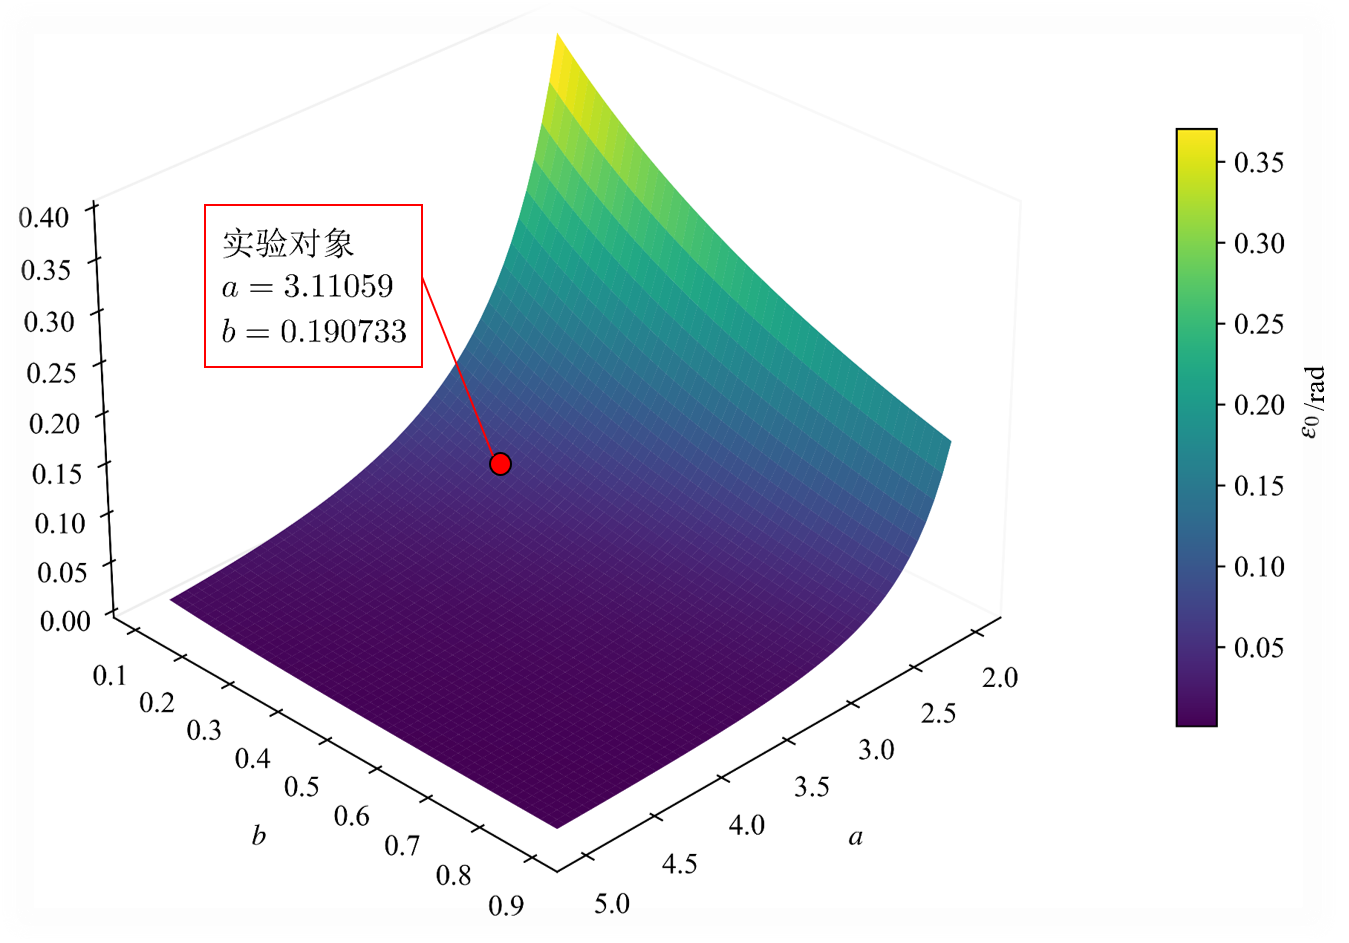
\includegraphics[width = 8cm]{./fig/epsilon_0.png}
			\captionof{figure}{$\varepsilon_0$的数值解可视化3D图，可以看出，当$a$和$b$越小（$I_1,I_2,I_3$越接近），$\varepsilon_0$越大，本文章的实验对象的相关数据已在图中标出. \label{fig:epsilon_0}}
		\end{center}
		
		以下是我们绘制的本文章的实验对象的$\varepsilon$热图.
		\begin{center}
			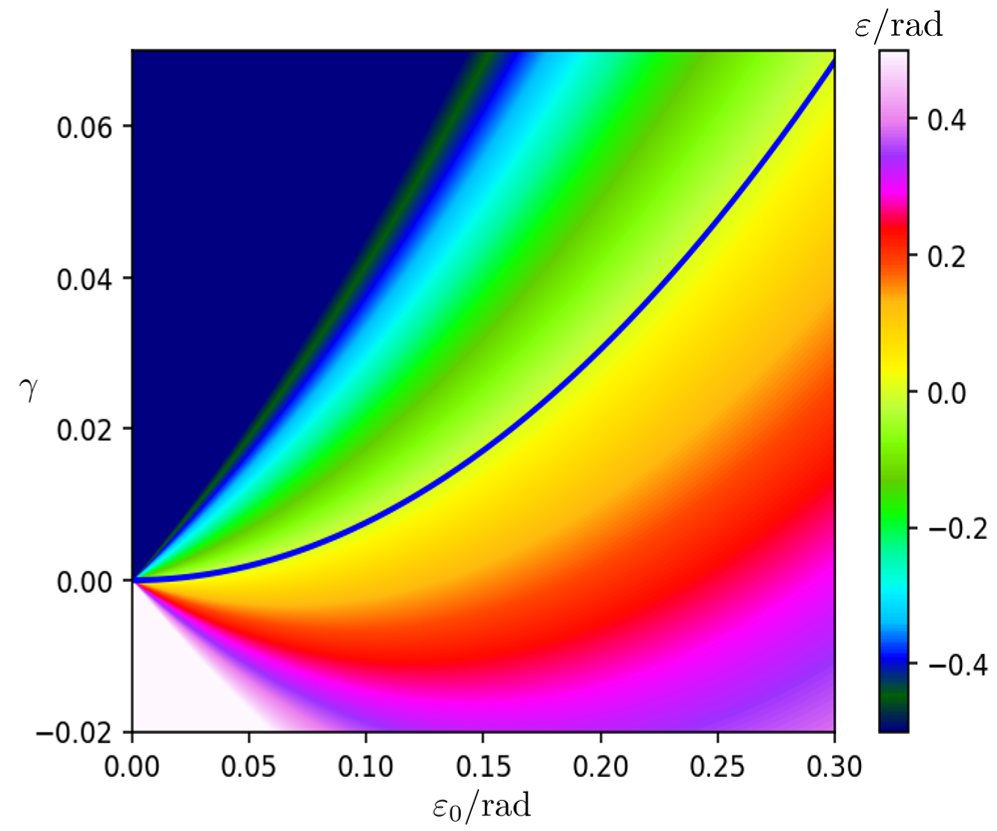
\includegraphics[width = 8.5cm]{./fig/epsilon.png}
			\captionof{figure}{$\varepsilon$的热图. \label{fig:epsilon}}
		\end{center}
		
		这个定理巧妙且成功指出了网球拍定理的本质，那就是当刚体整体在空中翻转一圈后（$\phi$转过近似$2\pi$后），此刚体翻面（$\psi$转过近似$\pi$），只不过此处是把目光放到$\phi$角旋转$2\pi$的误差$\varepsilon$，根据系统的连续性，若$\varepsilon$很小，大多数时候可以认为整体翻转完整一圈之后$\psi$的误差很小.
		
		\section{实验与计算模拟}
		我们在此部分将详细说明我们数据处理、初值问题计算、关于理论的数值预测和理论\autoref{thm:TRE}预测的对比进行详细叙述.
		
		\subsection{实验对象}
		首先讨论刚体的选用，在本次讨论中，鉴于条件有限，我们选用智能手机(vivo X200 pro mini)来进行分析，实验方法和数据收集软件的选取均主要参考于此文献\cite{2021_Wheatland}，软件是phyphox(RWTH Aachen University)，我们主要使用其陀螺仪的功能，其基础参数如下.
		\begin{center}
			\captionof{table}{实验对象参数}
			
			\begin{tabular}{>{\small}l >{\footnotesize\raggedright\arraybackslash}p{3.6cm}}
				\toprule
				项目 & 参数 \\
				\midrule
					单轴角速度上限 & $34.9063  rad/s$\\ \hline
				分辨率 & $0.0011  rad/s$\\ \hline
				延迟范围 & $2.500 ms \sim 2.500ms + 2.3850\times10^{-6}s$ \footnote{此处的1s延迟为设备标注的最大延迟，但是实际实验数据表明这个延迟主要在$2.500ms$小数点后三位之内浮动，在18635次计数中，延迟浮动的最大值为$2.3850\times10^{-6}s$，故几乎可以直接认为数据采集频率为400hz}\\ \hline
				手机质量(包括手机壳) & $216.4g$\\ \hline
				手机尺寸 & $155.0mm\times 76.0mm \times 9.510mm$\\
				\bottomrule
			\end{tabular}
		\end{center}
		
		\subsection{实验数据处理}
		
		数值处理我们是以能量和角动量为基础进行挑选，由我们实验数据结果图片可以看出，在实验过程中（即实验对象在空中进行旋转的时候）能量和总角动量大小几乎没有改变，而抛起和落地的时候能量呈现非常具有特征性的变化，主要体现为快速升高－平稳－突变（接到实验对象或者落到缓冲垫上）的过程，我们在检查实验数据是否到实验对象的最高测量上限以及审查整个实验过程中测量时间间隔和参考值的差别后选择了这段实验数据作为理论对比的对象.
		
		\begin{center}
			\includegraphics[width = 8cm]{./fig/minimal_axis.png}
			\captionof{figure}{实验数据.}
		\end{center}
		
		\begin{center}
			\includegraphics[width = 8cm]{./fig/energy_momentum.png}
			\captionof{figure}{实验对象的质心转动动能. \label{fig:energy_momentum}}
		\end{center}
		
		
		\subsection{算法综述}
		在选择模拟算法上，根据我们之前的分析，我们可以知道这个微分方程具备以下几个重要特征：
		\begin{itemize}
			\item 由中间轴定理，我们知道当我们以中间轴的旋转加上一些小扰动为初值之后，在固定点（即完美旋转的角速度在的位置）附近偏离的时候呈现指数增长，这对我们算法的选择提出了挑战，基础算法会在此处产生很大的误差，我们认为我们最后选择的算法至少是需要有自适应步长等处理局部快速变化的能力的.
			\item 此外，在空中的旋转具备两个非常关键的守恒量，分别是能量守恒和总角动量守恒，若是常规算法很可能导致误差积累，后期的误差越来越大，直接偏离了物理现实，如果要顾及本特征，我们最好选择具有辛方法特征的算法，这和第一个特征在我们选择算法方面在一定程度上有所矛盾，因为我们的基础常识是辛方法在误差方面表现不好，误差阶数不高，尤其是本微分方程具备指数增长阶段，这很可能导致算法误差过大，但是选择常规高阶自适应算法之后可能在一定时间之后呈现偏离，因为其在守恒量上表现不好.
		\end{itemize}
		我们首先使用基础欧拉法，以明确展示这些基础特征带来的影响，以下是我们用基础欧拉法计算得来的能量变化和角速度的相图，可以看出能量变化显著、相图曲线不闭合.
		
		\begin{center}
			
\includegraphics[width = 8cm]{./fig/E_euler.png}
			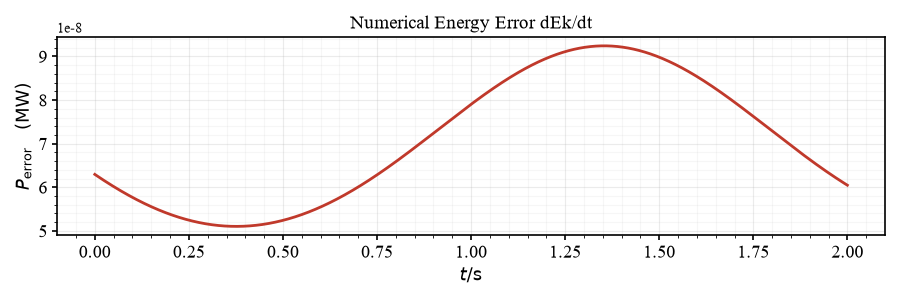
\includegraphics[width = 8cm]{./fig/dE_euler.png}
			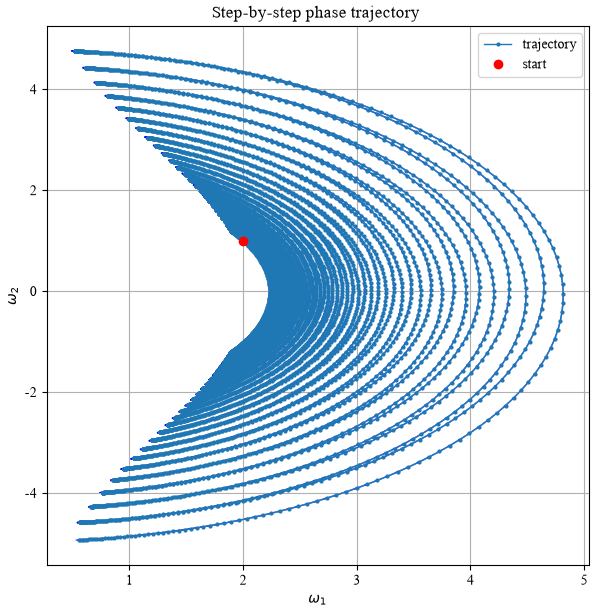
\includegraphics[width = 8cm]{./fig/phase_euler.png}
			\captionof{figure}{欧拉算法.\label{fig:euler_method}}
		\end{center}
		
		所以我们要采用更高阶且具有特殊方法保证守衡量不变的算法，以下是我们所在此问题中采用的算法综述：
		
		\begin{figure*}[!t]
			\centering
			
\includegraphics[
			width=\textwidth,
			keepaspectratio
			]{./fig/compare_E.png}
			\caption{能量图像，在能量和角动量图中我们把角动量中的$\omega_3$放到了里面，高阶自适应步长算法在剧烈变化（指数级增长和衰减）的时候呈现的能量波动以及波动后的能量的变化十分显著且对应关系明确.}
			\label{fig:method_compare}
		\end{figure*}
		
		\begin{itemize}
			\item \textbf{RK45}：显式自适应步长 Runge--Kutta 方法，通过四阶和五阶嵌套公式估计局部误差，并自动调整积分步长，在保证积分精度的同时提高计算效率。
			
			\item \textbf{DOP853}：八阶 Dormand--Prince 自适应 Runge--Kutta 方法，具有更高的积分精度和更好的误差控制能力，适用于高精度常微分方程数值求解.
			
			\item \textbf{Implicit Midpoint}：二阶隐式中点辛积分方法，能够保持系统的辛结构，在长时间积分过程中具有良好的能量和角动量守恒性能.
			
			\item \textbf{Gauss--Legendre 4 (GL4)} \cite{2006_Lubich_BOOK,2009_Ernst_BOOK}：四阶两阶段 Gauss--Legendre 辛积分方法，兼具高阶精度和辛结构保持特性，适用于刚体动力学等哈密顿系统的长期数值模拟.
			
			\item \textbf{Adaptive GL4 + Projection} \cite{2006_Lubich_BOOK,2009_Ernst_BOOK}：基于四阶 Gauss--Legendre 辛积分，引入自适应步长控制和流形投影技术，在提高积分效率的同时，将数值解投影回守恒流形，以保持系统能量和总角动量等守恒量.
		\end{itemize}
		
		以下是我们给出的关于欧拉动力学方程的模拟：
		
		\begin{center}
			
\includegraphics[width = 8cm]{./fig/compare.png}
			\captionof{figure}{多种算法绘制出的系统演化图像，良好的重合了.}
		\end{center}
		
		重点在\autoref{fig:method_compare}，RK45和DOP853两个高阶算法出现了显著问题，纵使算法阶数很高，但是在能量守恒方面仍然会受到明显的指数衰减和增长的冲击，从图中可以看出，在系统到达指数增长区间（中间轴定理起效）也就是顶峰的时候，能量会发生显著的波动，即第二张图的成簇波动，在没有指数增长或衰减的情况下，算法表现良好，能量几乎不变，但是一旦到达指数增长或衰减区间，能量会在短时间内剧烈波动后显著降低，整体呈现阶梯式下降，这也就是本微分方程如前所述的特殊之处，我们做出判断：
		
		高阶自适应算法无法胜任处理本方程的初值问题的工作.
		
		我们先不看RK45和DOP853，检查后面3种结合了辛积分的方法：
		
		\begin{center}
			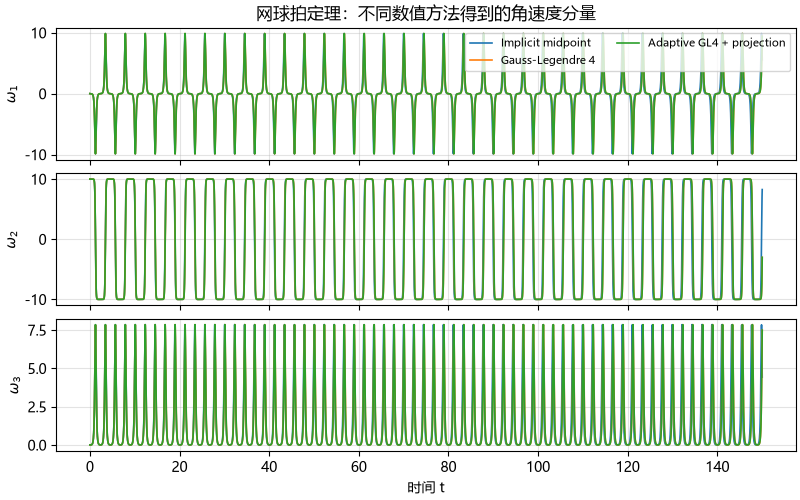
\includegraphics[width = 8cm]{./fig/final3.png}
			\captionof{figure}{长时间后的情况，没有显著区别，并且能量近乎不变，能量图像仅为一条直线，在有意义的范围内几乎无波动.\label{fig:final3}}
		\end{center}
		
		\begin{center}
			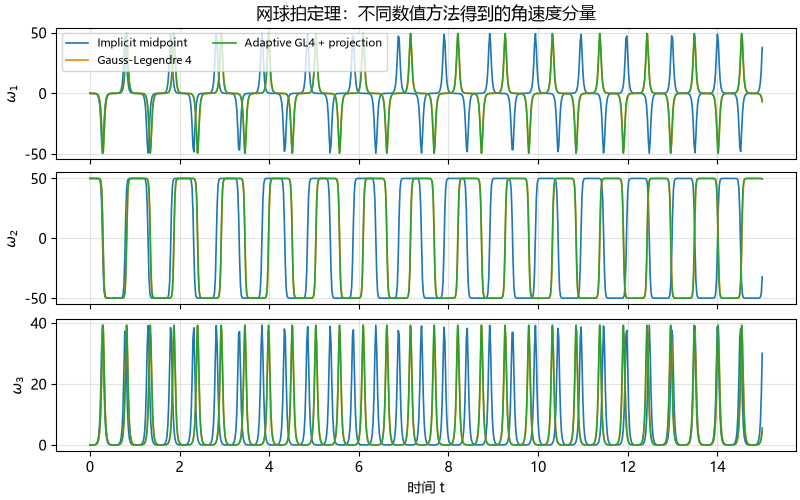
\includegraphics[width = 8cm]{./fig/final3_enhanced.png}
			\captionof{figure}{增大初始值的情况，在一段时间后算法预测的角速度结果出现劈裂（橙线和绿线是重合的），能量仍然很好地被保持了.\label{fig:final3_enhanced}}
		\end{center}
		
		由增大初始值之后产生的劈裂可以得知，虽然隐式中点辛积分能够保持角动量和能量守恒，但是其精度有限，并且隐式算法比较保守（以被预测的点作为变化率的计算点），在具有一定大小的初值的情况下经受不住局部指数变化的冲击，导致整体变化过快.
		
		我们对三种辛方法做出优缺点总结：
		
		\begin{itemize}
			\item \textbf{Implicit Midpoint}
			\begin{itemize}
				\item \textbf{优点：}计算逻辑简单、算力消耗低、计算速度快，适合短时、低精度的快速试算场景.
				\item \textbf{缺点：}精度层级低，误差累积效应显著，无法适配长时间仿真、大振幅强振荡的刚体旋转场景，数值稳定性较差.
			\end{itemize}
			
			\item \textbf{Gauss--Legendre 4 (GL4)} \cite{2006_Lubich_BOOK,2009_Ernst_BOOK}
			\begin{itemize}
				\item \textbf{优点：}四阶高精度，保辛效果好，常规场景下数值误差极小，仿真结果可信度高.
				\item \textbf{缺点：}采用固定步长，算力利用率较低。刚体旋转存在剧烈振荡与平缓变化交替的过程，固定极小步长会造成平缓阶段算力浪费，固定较大步长则会放大振荡阶段误差；同时缺乏投影校正机制，浮点舍入误差会长期累积，超长时间仿真仍可能出现微弱守恒量漂移.
			\end{itemize}
			
			\item \textbf{Adaptive GL4 + Projection} \cite{2006_Lubich_BOOK,2009_Ernst_BOOK}
			\begin{itemize}
				\item \textbf{优点：}四阶高精度、自适应高效算力分配，并结合投影校正保证物理守恒.
				\item \textbf{缺点：}需要进行步长迭代、误差估计以及约束方程求解，单步计算逻辑较为复杂，算力成本最高，并且非完全辛方法，大规模的调节步长会出现能量偏移，详情见后文.
			\end{itemize}
		\end{itemize}
		
		我们最后给出误差表格\autoref{tab:error}
		
		\begin{figure*}[!t]
			\centering
			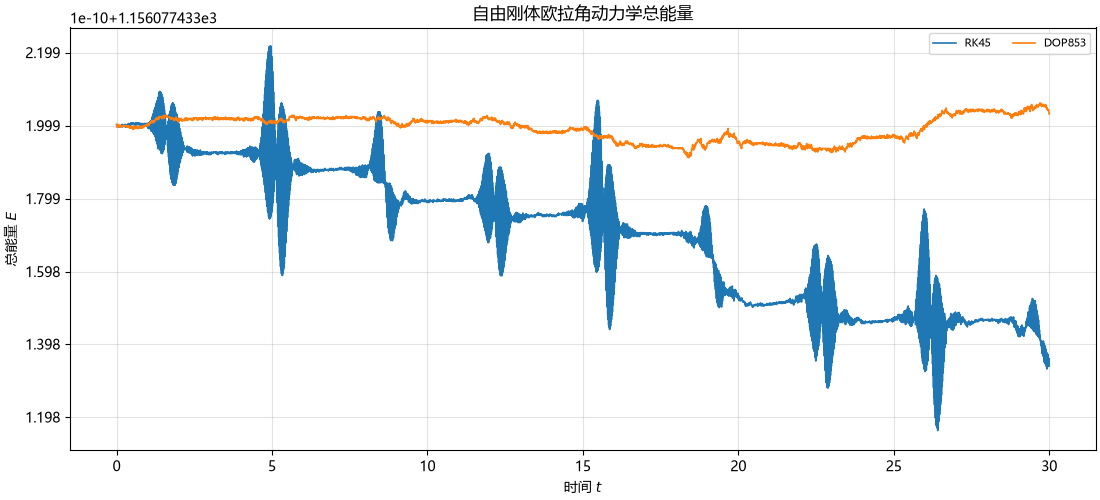
\includegraphics[
			width=\textwidth,
			keepaspectratio
			]{./fig/euler2_E.png}
			\caption{进一步去除所有辛方法的曲线，RK45特征与前面的图差不多，但是量级远小于辛方法，同时表现最为优秀的是DOP853，其能量变化有非单调的特征存在，加之其误差本就很小，使其能量变化相当少.}
			\label{fig:euler2}
		\end{figure*}
		
		\begin{table*}[t]
			\centering
			\caption{算法误差表格}
			\begin{tabular}{lcc}
				\toprule
				方法 & 最大能量误差/$\mu$J & 最大总角动量误差/Kg$\cdot$mm$^2 \cdot$s$^{-1}$\\
				\midrule
				RK45 & $1.37\times10^{-8}$ & $6.86\times10^{-9}$\\
				DOP853 & $3.76\times10^{-9}$ & $1.88\times10^{-9}$\\
				Implicit Midpoint & $3.51\times10^{-15}$ & $1.67\times10^{-15}$\\
				Gauss--Legendre 4 & $4.18\times10^{-15}$ & $2.30\times10^{-15}$\\
				Adaptive GL4 + Projection & $\mathbf{1.17\times10^{-15}}$ & $\mathbf{6.27\times10^{-16}}$\\
				\bottomrule
			\end{tabular}
			\label{tab:error}
		\end{table*}
		
		我们随后又用相同的方法探索了带入了欧拉角之后的欧拉动力学方程，但是最后给出了截然不同的结果\footnote{角动量的误差过小，并且可能截断误差非常显著，我们这里仅讨论能量的情况}：
		
		\begin{center}
			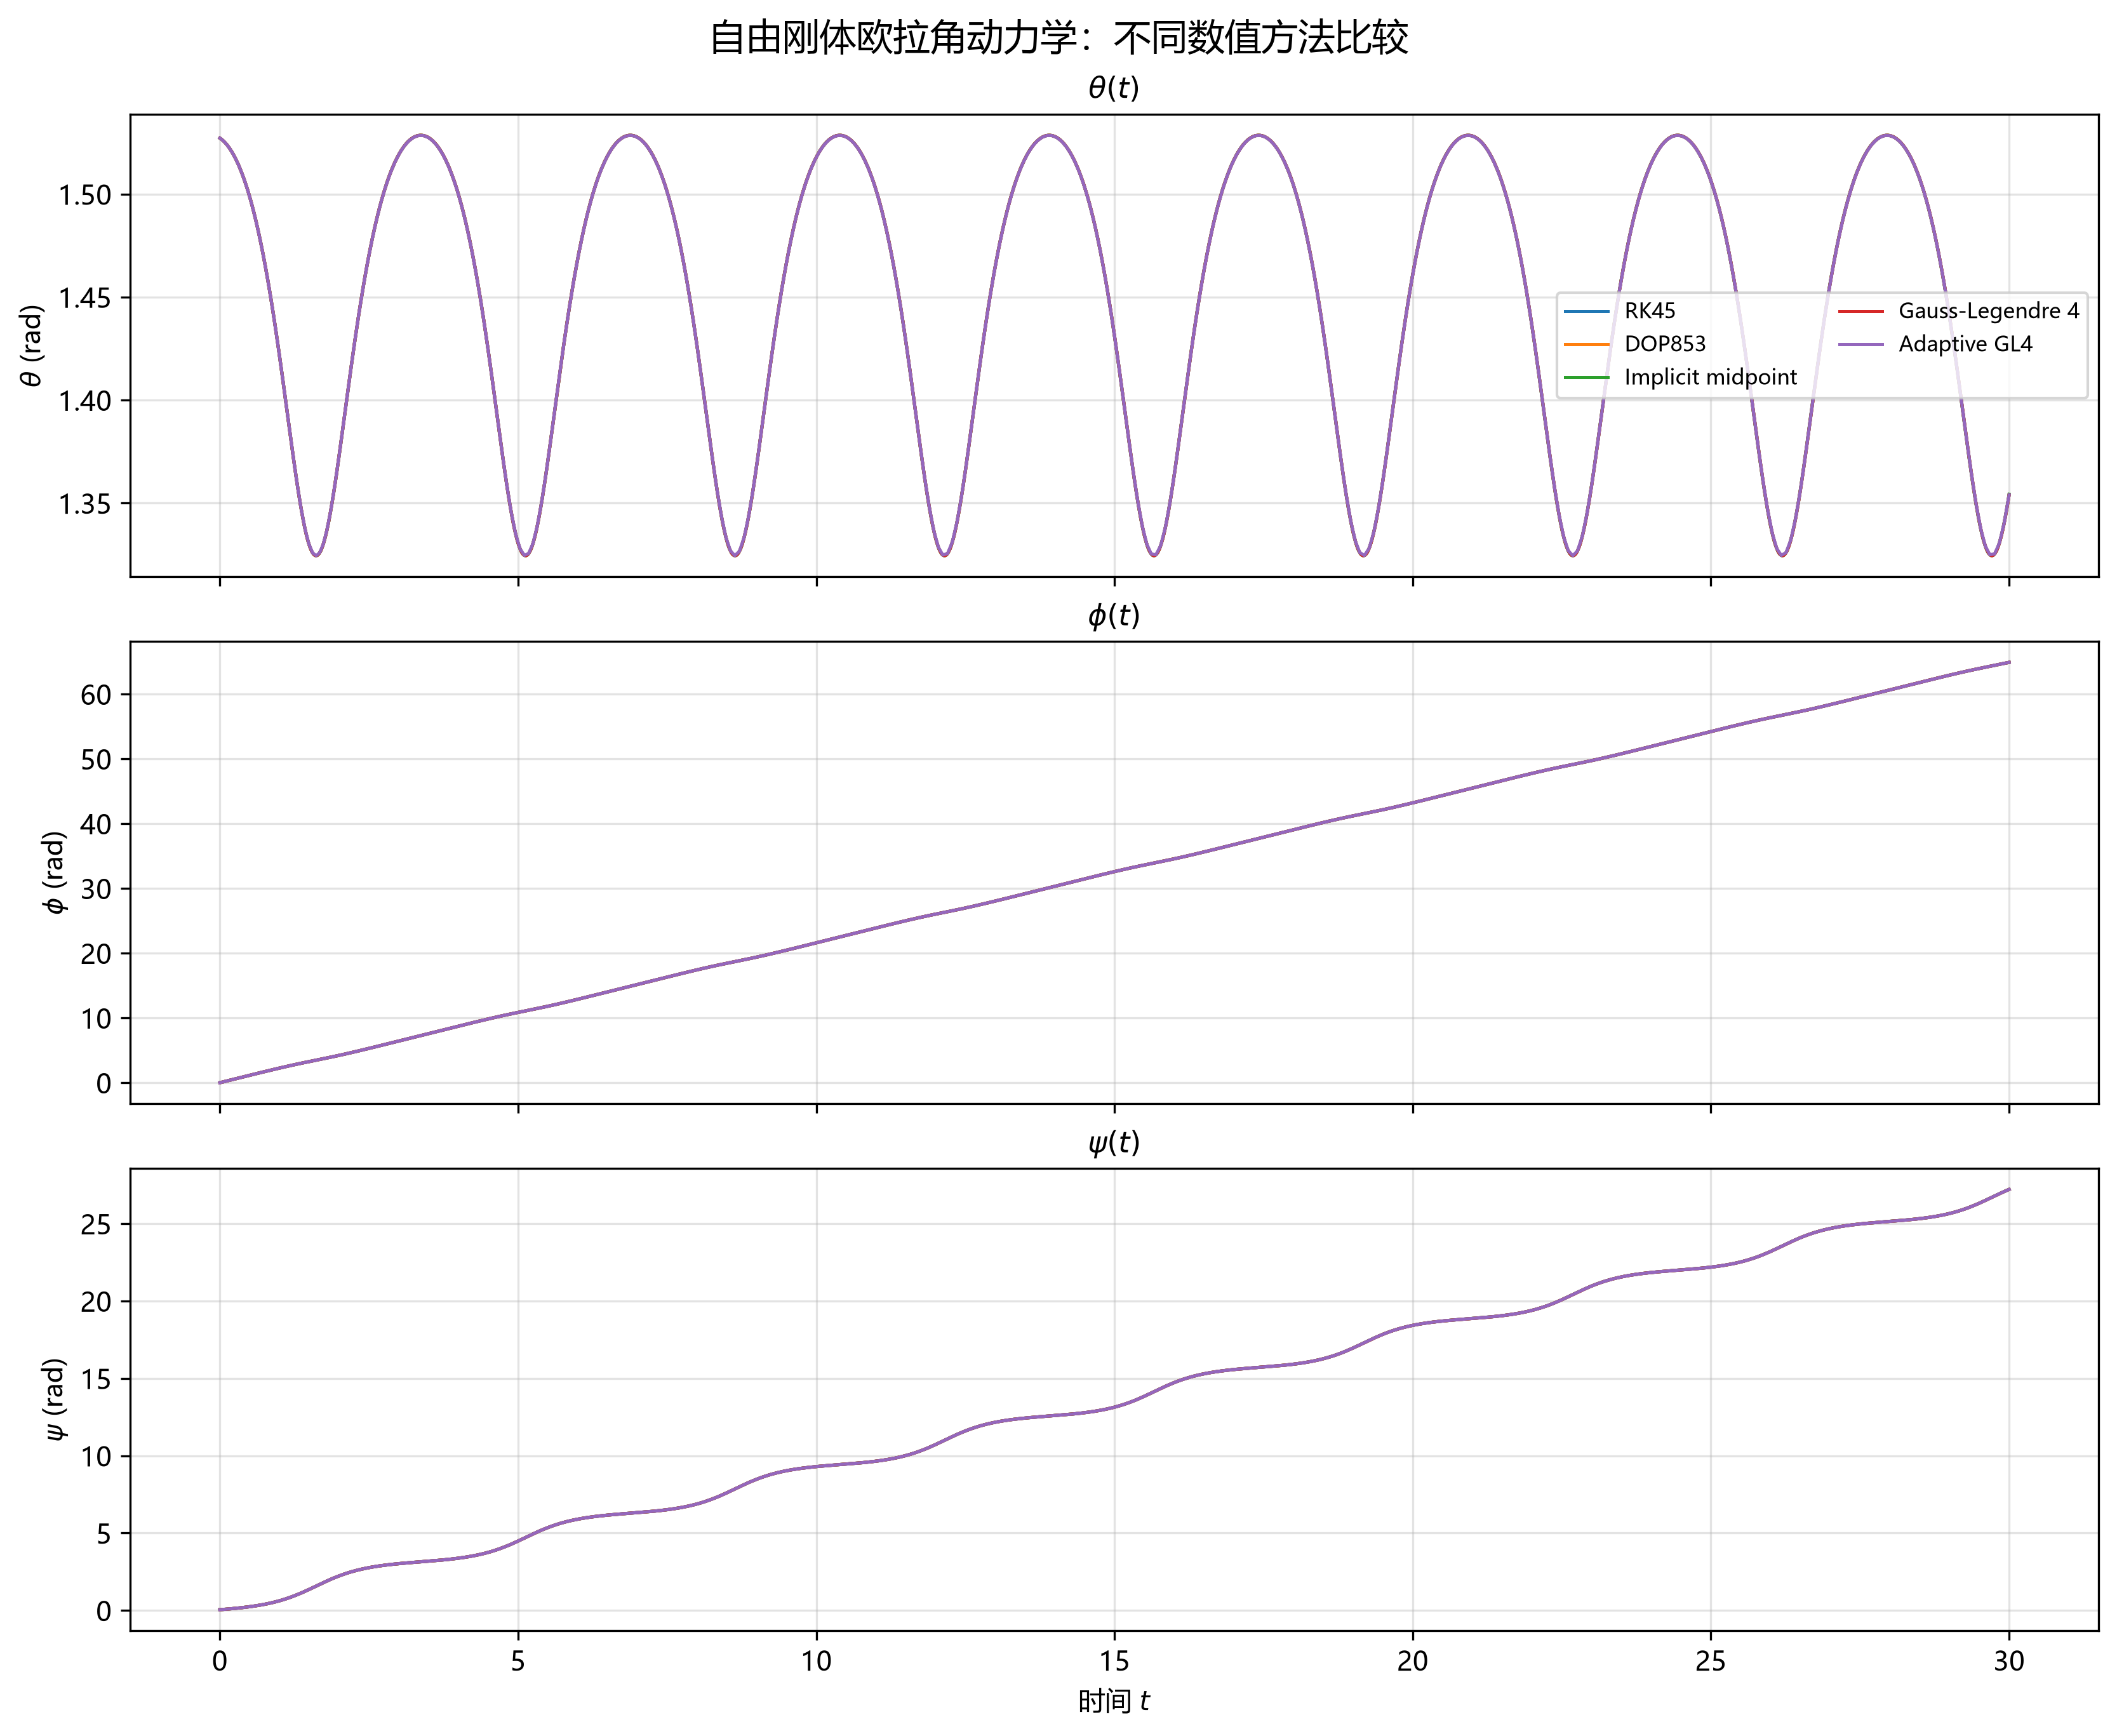
\includegraphics[width = 8cm]{./fig/euler_all.png}
			\captionof{figure}{欧拉角的数值解，与相图中的转动状态一致.\label{fig:euler_all}}
		\end{center}
		
		\begin{center}
			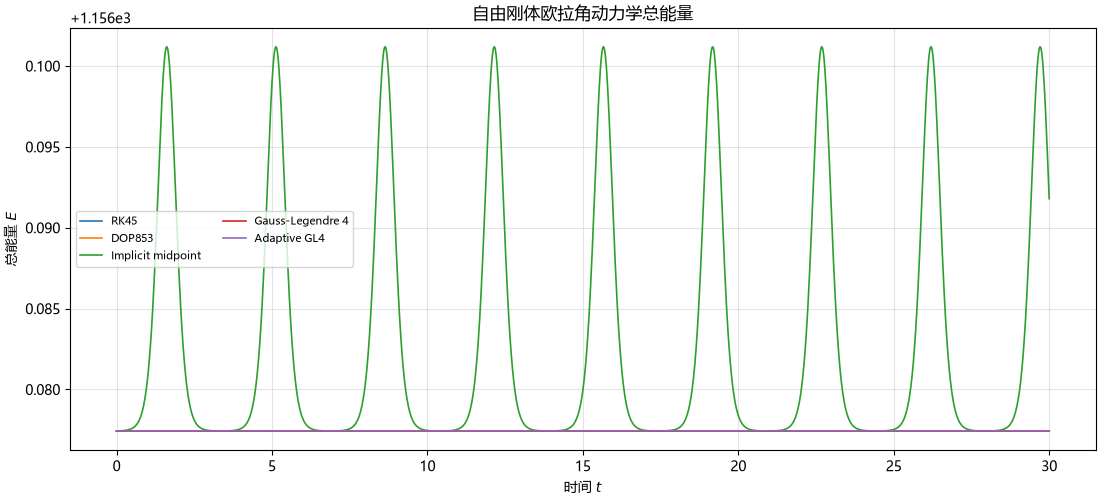
\includegraphics[width = 8cm]{./fig/euler_all_E.png}
			\captionof{figure}{欧拉角的数值解，隐式中点辛积分能量误差呈现周期性且非常大，我们在尝试不同总角动量和不同时间长短之后效果一致.\label{fig:euler_all_E}}
		\end{center}
		
		\begin{center}
			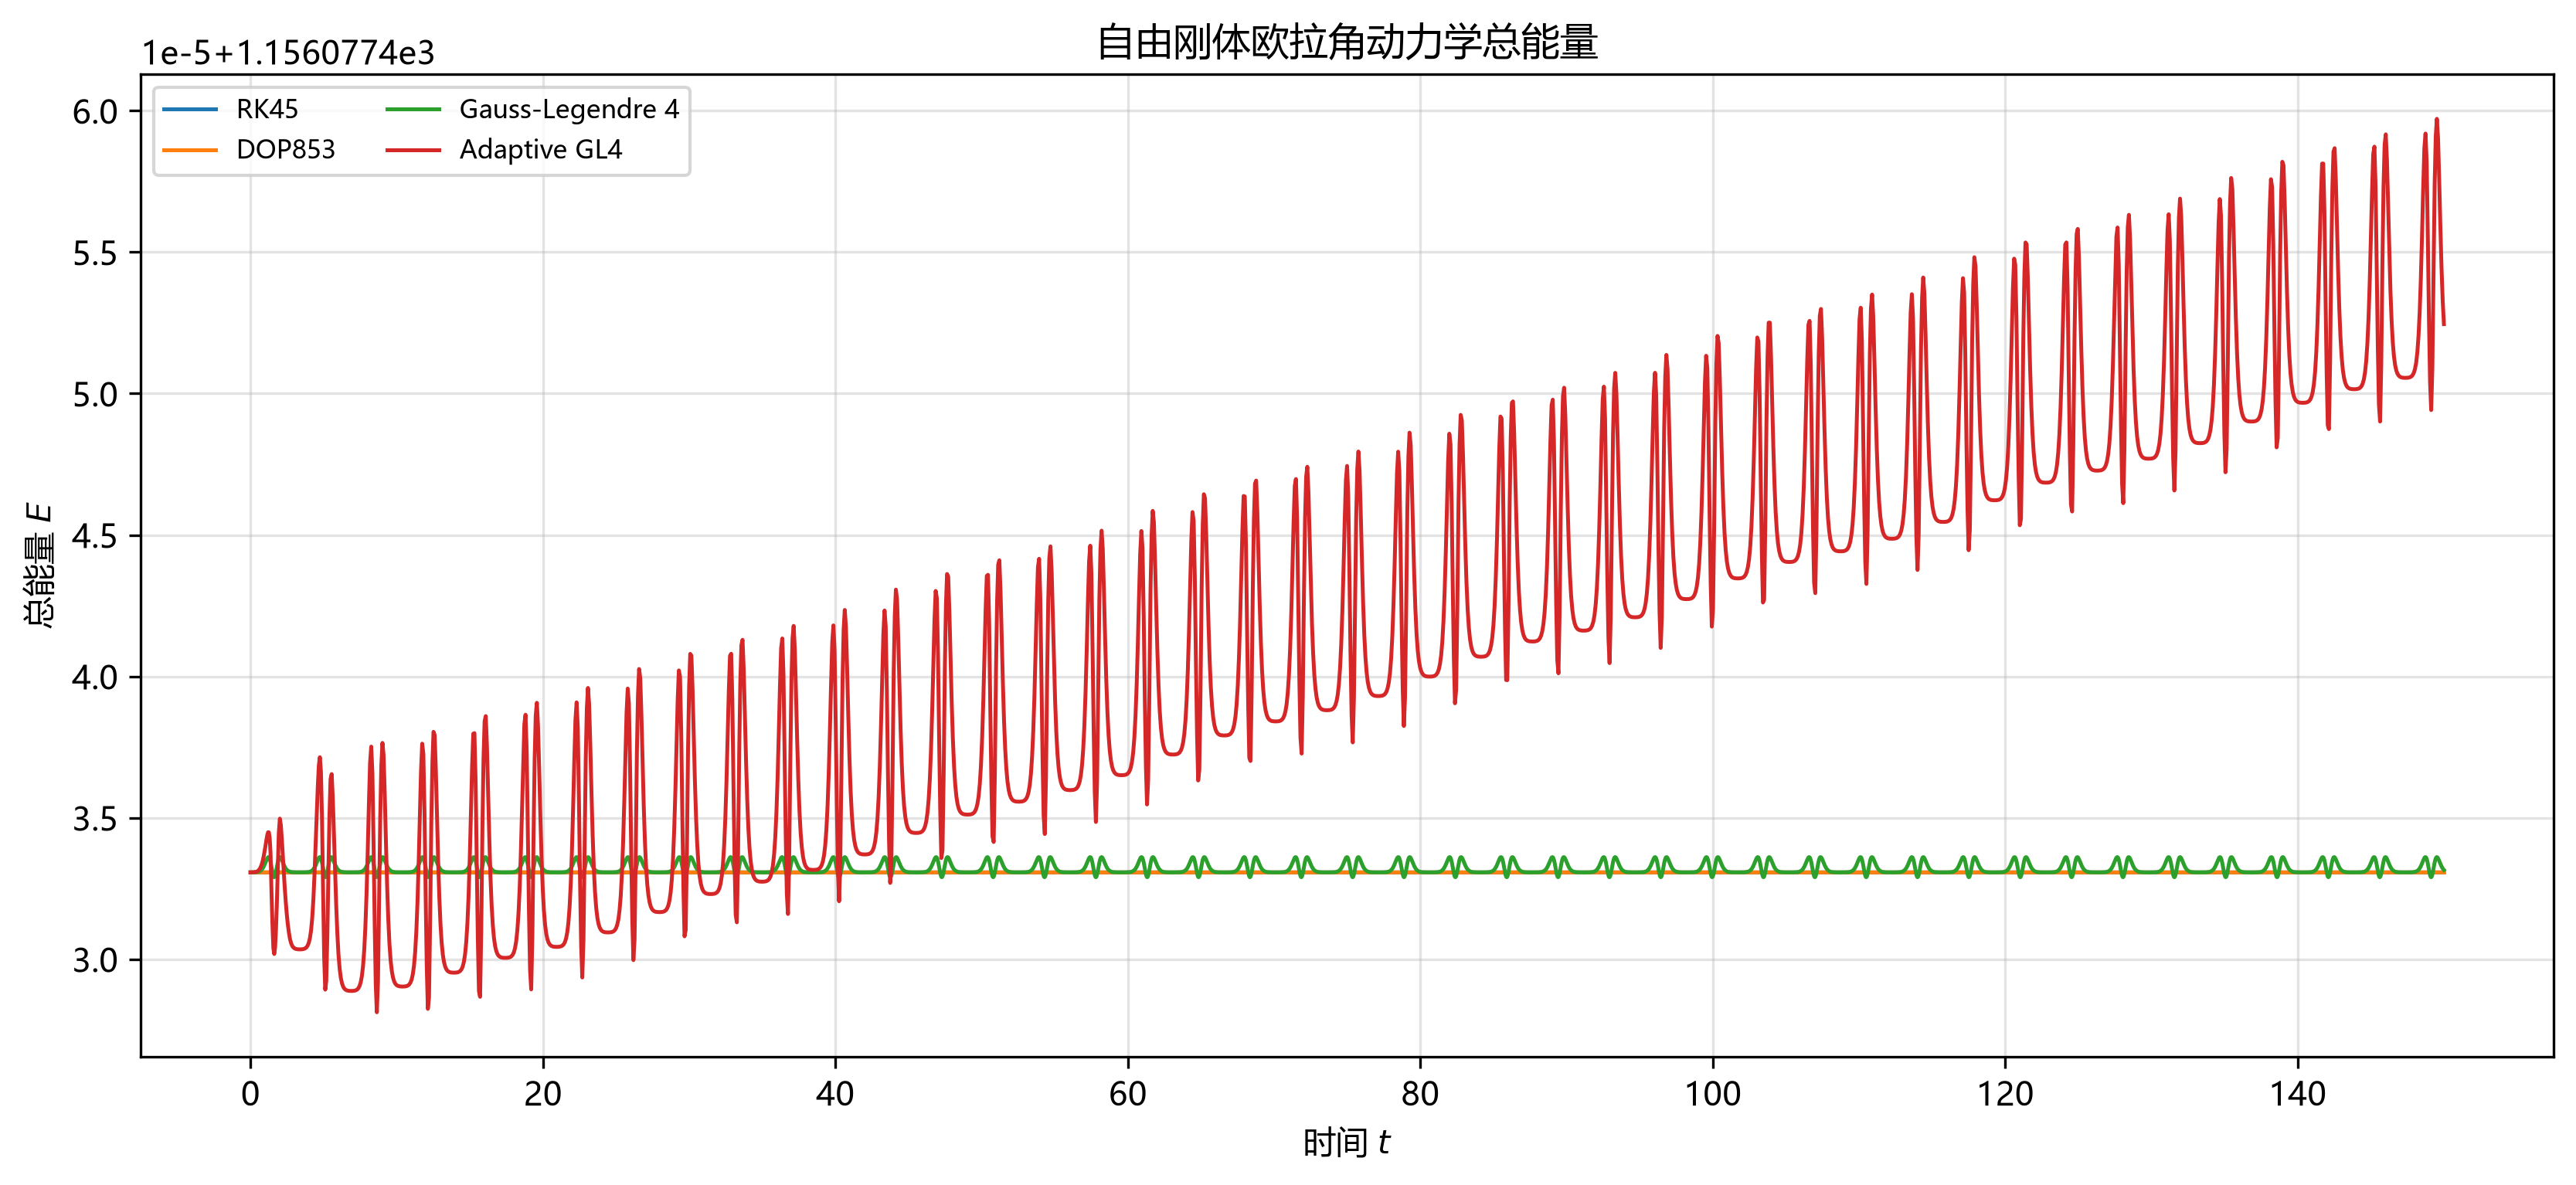
\includegraphics[width = 8cm]{./fig/euler_longtime.png}
			\captionof{figure}{去除隐式中间点，拉长时间范围，注意到一开始表现最好的Adaptive GL4不但误差大且逐渐偏离，我们最后会简要说明.\label{fig:euler4}}
		\end{center}
		
		\begin{center}
			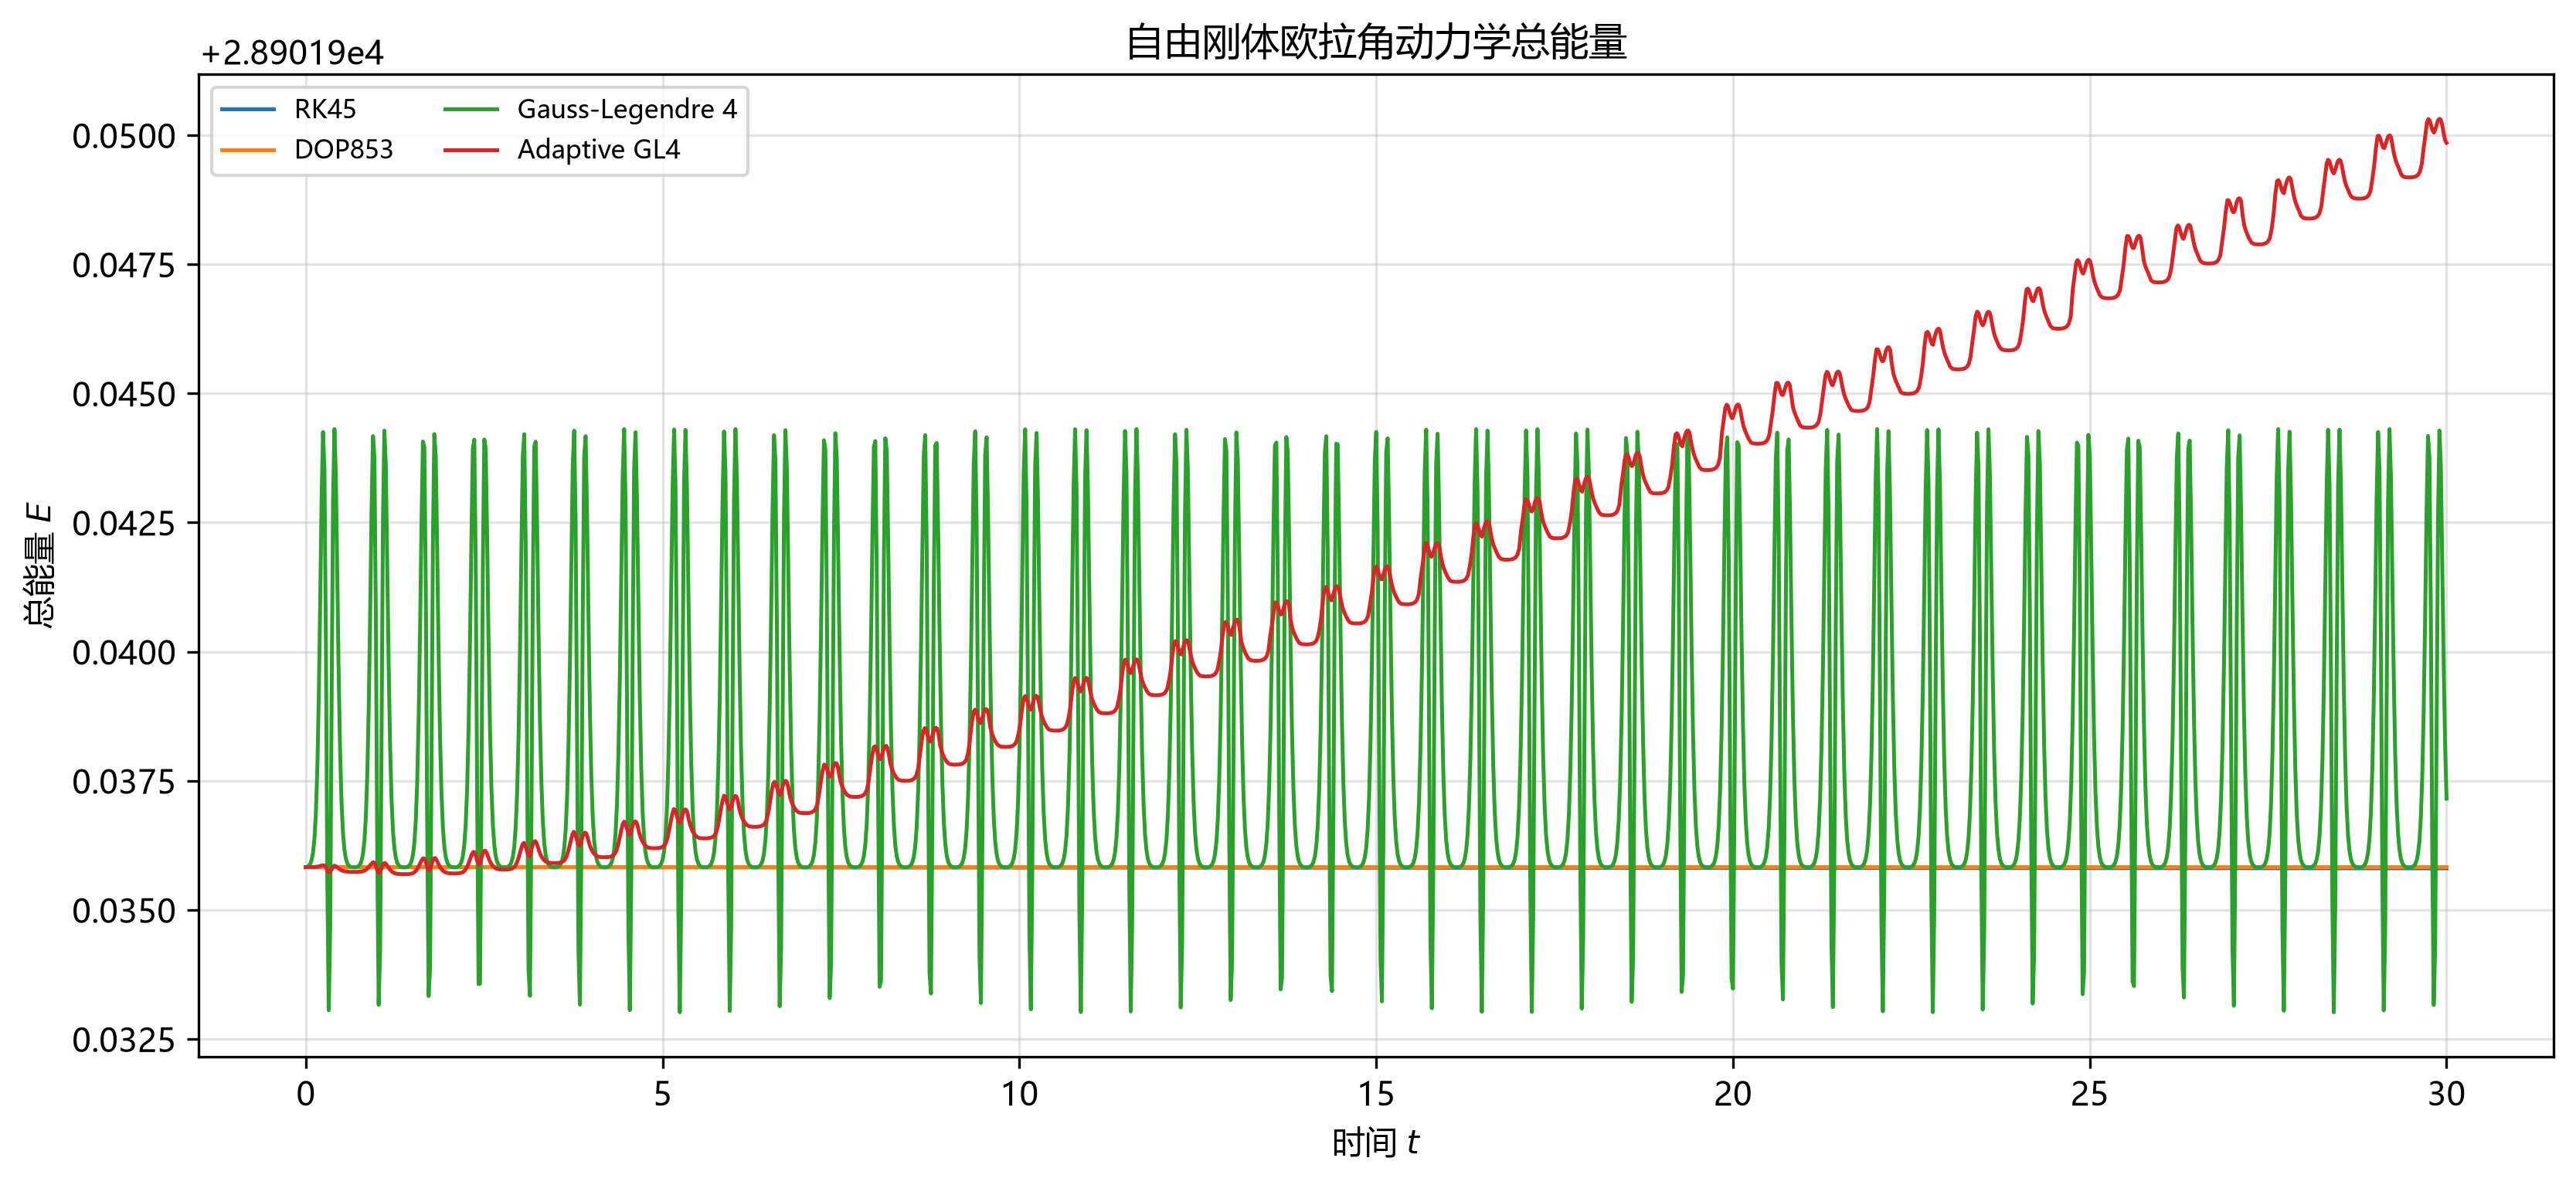
\includegraphics[width = 8cm]{./fig/euler_enhance.png}
			\captionof{figure}{提高初值大小，我们发现此处GL4的误差对于初值的大小十分敏感，这可能是由于其精度阶数很低导致快速变化对其的冲击远大于其他算法，而Adaptive GL4由于有自适应步长，就很好地减少了此冲击的效果.\label{fig:euler_enhance}}
		\end{center}
		
		从中可以看出高阶算法在这种情况虽然有局部震荡，但是整体误差远小于辛方法（$5\sim 10$个量级），可以看到辛方法（即使有高阶算法提升）在面对时间范围不是很大的问题时，其对快速变化仍旧很脆弱，辛算法在阶数上的提升确实能够在一定程度上提升其精度，但是相比于自适应步长高阶算法来说仍然带来了不小的误差（5个量级）.
		
		而高阶算法虽然与前面的问题一致，存在强烈的局部震荡，也只是相对预期已经积累的偏差而言，实际上最后带来的误差仍然不会过大，在此问题背景下，高阶自适应步长算法如果要产生比辛算法更大的能量偏差，就至少要积累此处展示的时间长度的4、5个量级.这与前面的结果截然相反.
		
		主要是因为在前面的结果中，指数增长结合在高阶自适应步长算法中带来的能量误差远大于辛方法，而这里效果相反，这说明快速变化对辛方法和高阶算法带来的影响不是线性的，即依据方法和方程的形式而不同，我们此处没有改变计算的物理模型的本质，仅仅是带入了欧拉角、更改初值或拉长时间，最后能量波动的结果截然不同.
		
		但是归根结底算法的特征是一致的，高阶算法仍然保证了其高精度性，以及能量误差的单调性，同样也呈现阶梯式下降，辛方法仍是在局部进行波动，不过值得一提的是，Adaptive GL4在这里出现了上升的情况，这是因为Adaptive GL4不是严格的辛积分器，这在书籍\cite{2006_Lubich_BOOK}有复杂且严格的讨论，我们不做深入分析.
		
		\begin{center}
			\captionof{table}{替换欧拉角之后的算法误差表格}
			
			\begin{tabular}{>{\small}l >{\footnotesize\raggedright\arraybackslash}p{3.6cm}}
				\toprule
				方法 & 最大能量误差/$\mu$J \\
				\midrule
				RK45 & $7.26\times10^{-14}$ \\
				DOP853 & $7.87\times10^{-15}$ \\
				Implicit Midpoint & $2.06\times10^{-5}$ \\
				Gauss--Legendre 4 & $4.67\times10^{-10}$ \\
				Adaptive GL4 & $\mathbf{6.22\times10^{-9}}$ \\
				\bottomrule
				\label{tab:euler_error}
			\end{tabular}
		\end{center}
		
		\subsection{总结}
		于此我们完整对比了多种初值问题，计算方法，即对于一个复杂并且具有两个似乎矛盾的特征的微分方程的求解，可以看出不只是对于不同的问题，甚至是对于同一个问题，不同形式下的方程，每一个算法都会带来截然不同的误差大小，虽然他们都保持了自己原来算法的特征，但是所带来误差的大小却因为两个复杂因素而难以断定哪个方法更合适，在此背景下，具体选择哪种方法需要看方法实际的表现来决定.
		
	\section{结论与未来展望}
	在本篇文章中，我们全面描述了网球拍效应的理论说明和可视化展示，并提供了相图、全面的描绘了系统的演化过程，同时我们指出本方程同时具备两个守恒量和剧烈变化区间，采用了多种不同的方法进行，尤其是对比了辛方法和高阶方法在本系统中的表现，在相同系统的方程的两种不同的变量形式下两批算法的精度截然不同，提醒了我们在未来面对快速变化和具有多个守恒量的系统时，应结合多个算法的具体表现做出判断，本文章的不足之处在于对比的算法数量有限，而且对比仅限在本问题之上，没有把算法施加到其他具有相同特征的系统上面进行更广泛的研究，结论有待精炼和推广，我们在这一方面期待未来的进一步研究.
	
		
%-----------------------显示参考文献------------------------%
        \bibliographystyle{thuthesis-numeric}%这里使用了清华大学学位论文模板样式，其与《大学物理》期刊官方论文模板要求一致
       		\nocite{*}%让所有未被引用的文献都列出
        \bibliography{./bib/clgpy}

    \end{multicols}%结束分栏

\newpage
%-----------------------英文信息部分------------------------%
\Title{Nonlinear Dynamic Analysis, Experiments, and Simulations of the Tennis Racket Effect}
\Author{XIA Jun-lin, DONG Hao, JIANG Cheng-yuan}
\Institute{(College of Physics and Astronomy, Yunnan University, Kunming 650504, China)}
\Maketitle
\begin{enabstract}
    This thesis focuses on the theoretical, experimental, and numerical investigation of the tennis racket theorem. From the theoretical perspective, the study primarily employs phase-space analysis in nonlinear dynamics to reveal the underlying mechanisms governing the instability of rigid-body rotation. Experimentally, angular velocity measurements are conducted in the body-fixed reference frame using a rigid body instrumented with angular velocity sensors, and the experimental results are systematically compared with theoretical predictions to validate the analytical model. In the numerical study, several integration methods for initial value problems are investigated and evaluated. Considering the unique characteristics of the tennis racket theorem, the advantages, limitations, and applicable scenarios of each numerical method are discussed in detail. The results presented in this thesis provide both a theoretical framework and representative numerical case studies for potential future applications involving rigid-body attitude dynamics and related engineering problems.
\end{enabstract}
\enkeywords{Nonlinear Dynamics; Phase Space Analysis; Initial Value Problems; High-Order Numerical Methods; Adaptive Step Size; Symplectic Integration; Rigid-Body Dynamics}


\end{document}
